% !TeX root = ../report.tex

\section{Trident Ray Theory} \label{sec:trident_theory}

Currently, there are many existing ray tracing algorithms for High-Intensity Focused Ultrasound simulation \cite{StochasticSim}. Most of them aim at computing the powerloss density (heat production) or intensity from beams of rays cast from a transducer. Two existing methods will be introduced briefly because they are the inspiration of the method used in this study.

The first method is to sum over all rays (set $\Phi$) that pass through a grid cube. Their energy loss in the cube is:

\begin{equation} \label{eq:first_rc}
    H = \sum_{a \in \Phi} (P(r_{a,in}) - P(r_{a,out})) = \sum_{a \in \Phi} P(r_{a,in})(1-e^{-2\alpha ||r_{a,in} - r_{a,out}||})
\end{equation}

Where $H$ is the total powerloss by all rays in the sampling grid, $\alpha$ is the attenuation factor. $r_{a,in}$, $r_{a, out}$ are the entry point  and exit point of the box on the ray, respectively. To obtain the powerloss density $Q$ (in $watt/m^3$), $H$ needs to be divided by volume. For each ray in $\Phi$, the algorithm needs to calculate the position where it enters and leaves a gridbox. This method cannot handle the situation where intersections are present.

In the second method, the rays are grouped into paths. Note that here same path only means that the rays start from the same transducer element, pass through the media in the same order and have the same properties such as wave type. Rays with the same path are treated as a bundle ($b$). Take the situation in Figure \ref{fig:one_gridbox} for example, the the value of the intensity loss for all the rays that follow the same path $b$ can be calculated from:

\begin{equation} \label{eq:calc_I_Loss}
    I_{loss,b}(\vec{r_c})=\sum_{a \in b} \frac{||\vec{r}_{a,in}-\vec{r}_{a,out}||}{\Delta V} P(\vec{r}_{a,in})
\end{equation}

From intensity loss $I_{loss}$, the pressure generated by all the rays in the same path $b$ can be calculated from:

\begin{equation} \label{eq:pressure_calculation}
    p_b(\vec{r}_c)=\sqrt{2\cdot Z\cdot I_{loss,b}(\vec{r}_c)e^{i\bar{\phi}_b}}
\end{equation}

Now accumulate the contribution of all the possible bundles $U$ to get the pressure $p_{tot}$:

\begin{equation} \label{eq:sum_all_bundle}
    p_{tot}(\vec{r}_c)=\sum_{b \in U}p_b(\vec{r}_c)
\end{equation}

Accroding to Modena et al \cite{Modena_2018}, the fluid heat production is given by:

\begin{equation} \label{eq:fluid_hp}
    Q(\vec{r})=\frac{\alpha}{Z}|p_{tot}|^2
\end{equation}

\begin{figure}
    \centering
    \begin{subfigure}[b]{0.45\textwidth}
        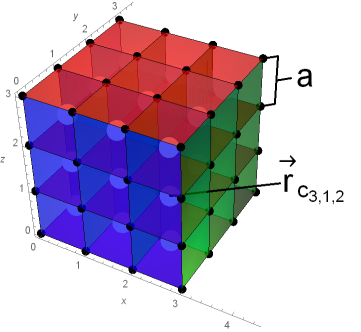
\includegraphics[width=\textwidth]{gridbox}
        \caption{}
        \label{fig:gridbox}
    \end{subfigure}
    %
    \begin{subfigure}[b]{0.5\textwidth}
        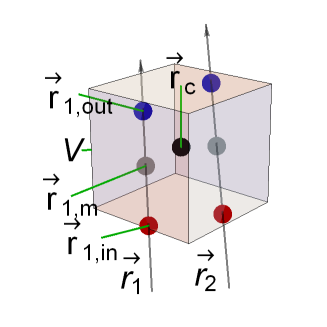
\includegraphics[width=\textwidth]{one_gridbox}
        \caption{}
        \label{fig:one_gridbox}
    \end{subfigure}
    \caption{(a) An example of Axis-Aligned Bounding Box (AABB) where $r_{c_{3,1,2}}$ is the center of the box $[3,1,2]$ (b) single box with intersection, $r_1$ enters the box at $r_{1,in}$ and exit at $r_{1,out}$, similar for $r_2$}
\end{figure}

By combining the equations \ref{eq:calc_I_Loss}, \ref{eq:pressure_calculation}, \ref{eq:sum_all_bundle}, \ref{eq:fluid_hp}, we can arrive at the equation for heat production calculated from ultrasonic rays at the center of the cube.

\begin{equation} \label{eq:heat_production_final1}
    Q(\vec{r}_c)=\frac{2\alpha}{V}\left|\sum_{b \in U}\sqrt{(\sum_{a \in U_b}P(\vec{r}_{a,in})\left\|\vec{r}_{a,in}-\vec{r}_{a,out}\right\|)} e^{i\bar{\phi}_b}\right|^2
\end{equation}

The flow of acoustic power from each transducer element is described by a number of rays\cite{sonalleve}. With more rays being sent out in the simulation, the intersection of each box tends to converge to a stable ratio. As can be seem from equation \ref{eq:heat_production_final1},in order to obtain the powerloss density, first, the impact of all the rays are accumulated within every path (bundle). For every path, their contribution is calculated in the outer summation. In a HIFU simulation, there can be many bundles due to reflection and refraction of the rays. This will cause the computation to be very expensive when a large number of rays are utilized to approximate the real intensity. 

A new idea is proposed by Prof. Dr. Ir. Huub ten Eikelder that instead of casting a large number of rays from the transducer to approximate the intensity, one can use the "trident" rays, each of which is the combination of three rays to keep track of the divergence of the beam. One of the three rays carrys the power information, the other two only serve to track the changes in area. These three rays have almost identical paths and the geometrical spreading can be tracked by the divergence of the ray pattern (Figure \ref{fig:Trident_ray}). At any sampling point, a plane perpendicular to the power carrying ray is created to intersect the three rays. The area of the triangle formed by the three intersection points is $S_1$ and can be used as how much the beam has spreaded. The power on a point along the ray is given by attenuation equation $P_1=P_0\cdot e^{-2\cdot \alpha \cdot r}$. Hence, the intensity and powerloss density can be derived from:
\begin{equation} \label{eq:calc_intensity}
    I=\frac{P_1}{S_1}
\end{equation}
The standard way to calculate powerloss is:
\begin{equation}
    Q=2\alpha I
\end{equation}

As the length on the ray increases, the area increases quadratically as well as the divergence of the beam. In theory, it requires only one ray per bundle to determine the intensity from this bundle. This method can achieve similar pricision with less rays, compared with the first method because it only requires that there's at least one intersection with the box per bundle.

However, in real simulation, it seldom happens that there's only one ray from a bundle that intersects a box. The contribution of the bundle to the pressure in this box will then be the average pressure from these rays. More detailed discuss is available in section \ref{sec:measurement}.

\begin{figure}[h]
    \centering
    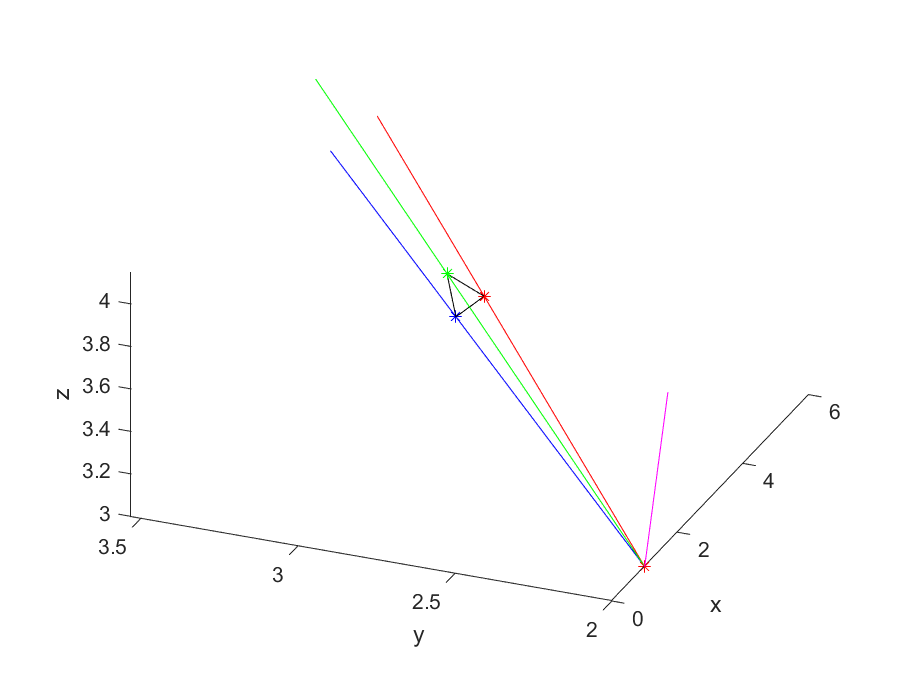
\includegraphics[width=0.6\textwidth]{trident.eps}
    \caption{An example of trident rays, the angle between rays are larger for demonstration purpose.}
    \label{fig:Trident_ray}
\end{figure}

%%%%%%%%%%%%%%%%%%%%%%%%%%%%%%%%%%%
\section{Components of HIFU Model} \label{sec:components}

An MR-HIFU system is a highly sophisticated system with many components. For simplicity reasons, the MR-HIFU system is modelled as being composed of only transducer, media, rays and sampling box. The model uses the actual geometry of the V2 phased array transducer of the Philips Sonalleve system \cite{sonalleve}, which consists of 256 elements placed on a spherical shell (12 cm radius of curvature and 13 cm aperture) operating at 1.2 and 1.4 MHz. The focus point created by this system is cigar shaped with dimensions of approximately 2 mm width and 7 mm length. The power of the transducer can be set as a parameter in the model, in this study, 256 watt (1 watt per transducer) is used as the total power of the transducer. 

\begin{table}[h!]
    \centering
    \begin{tabular}{c c c c c c c c} 
        \hline
        Medium & \textit{TH} & $c$ & $\rho$ & $\alpha$ & $c_p$ & $k$ \\ [0.5ex] 
        \hline\hline
        Oil & - & 1430 & 1070 & 1.04 & 4200 & 0.5 \\
        \hline
        Gel pad & 15 & 1580 & 1030 & 0.8 & 3600 & 0.65 \\
        \hline
        Skin & 2 & 1610 & 1200 & 50 & 3600 & 0.56 \\
        \hline
        Muscle & 10 & 1547 & 1050 & 9.8 & 3600 & 0.56 \\
        \hline
        Bone & - & 3736/1995 & 2025 & 1.9/2.8 & 3720 & 0.487 \\
        \hline
        Liver & - & 1578 & 1050 & 5.65 & 3600 & 0.56 \\
        \hline
    \end{tabular}
    \caption{Properties of the materials used in this study. \textit{TH}: thickness,  $c$: speed of sound, $\rho$: density,  $\alpha$: attenuation, $c_p$: specific heat capacity, $k$: thermal conductivity. \cite{Modena_2018} \cite{markoil}}
    \label{tb:media_property}
\end{table}

The transducer is submerged in Castor oil which has a very low attenuation factor for ultrasonic power (Figure \ref{fig:submerged_transducer}). The acoustic property of Castor oil is given by Ramaekers et al \cite{markoil}. The Castor oil is separated from the air by a thin membrane. The tissue is modeled as consisting of only bone and muscle. Skin and other soft tissues have very close properties to that of the muscle and thus are not discriminated. For ultrasonic waves, the muscle and the skin behave as a fluid and the bone behaves as a solid. By definition, propagation of shear (transversal) wave is only possible in non-fluid. Castor oil is the initial medium of the trident rays. 

\begin{figure}[h]
    \centering
    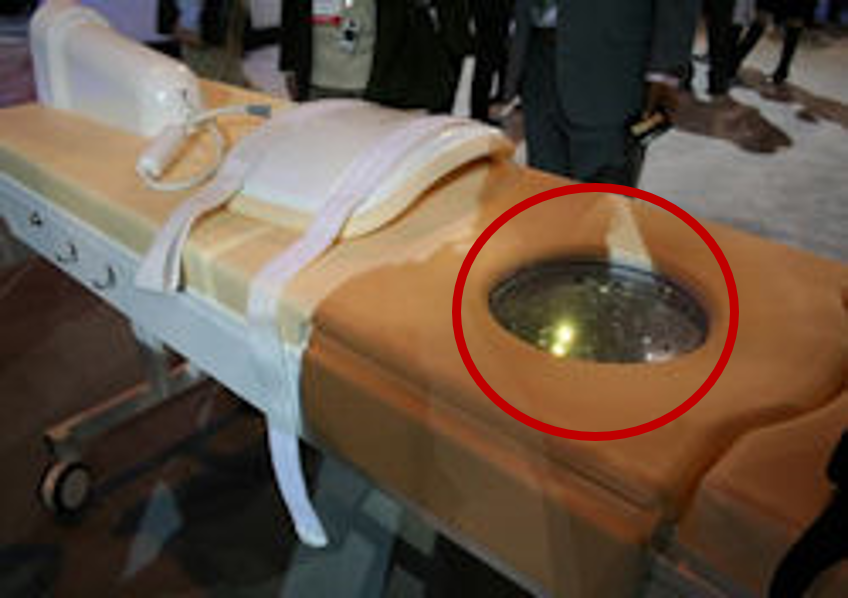
\includegraphics[width=0.5\textwidth]{transducer_markoil}
    \caption{Transducer element submerged in Castor oil (red circle) \cite{sonalleve} \cite{vanwijk2013}.}
    \label{fig:submerged_transducer}
\end{figure}

To measure the power production in the media caused by the ultrasound, a sampling box is employed (Figure \ref{fig:sampling_box}). Since many sampling points are required due to the small wave length, the sampling box is kept small, only around the focus region, which would also be the lesion area in therapeutic application. The box is divided into smaller cubes. The smaller the cubes are, the finer the resolution (Figure \ref{fig:gridbox}). The edges of the cubes should be larger than the ultrasound wave length. Two measurement methods are implemented. The first one uses the projection of the center of the cubes on the ray as the length to calculate intensity and add the intensity of all the rays together. The secound method differs from the first method only in that the summation is weighted based on the length of the intersection of the ray with the cubes.

\begin{figure}[h]
    \centering
    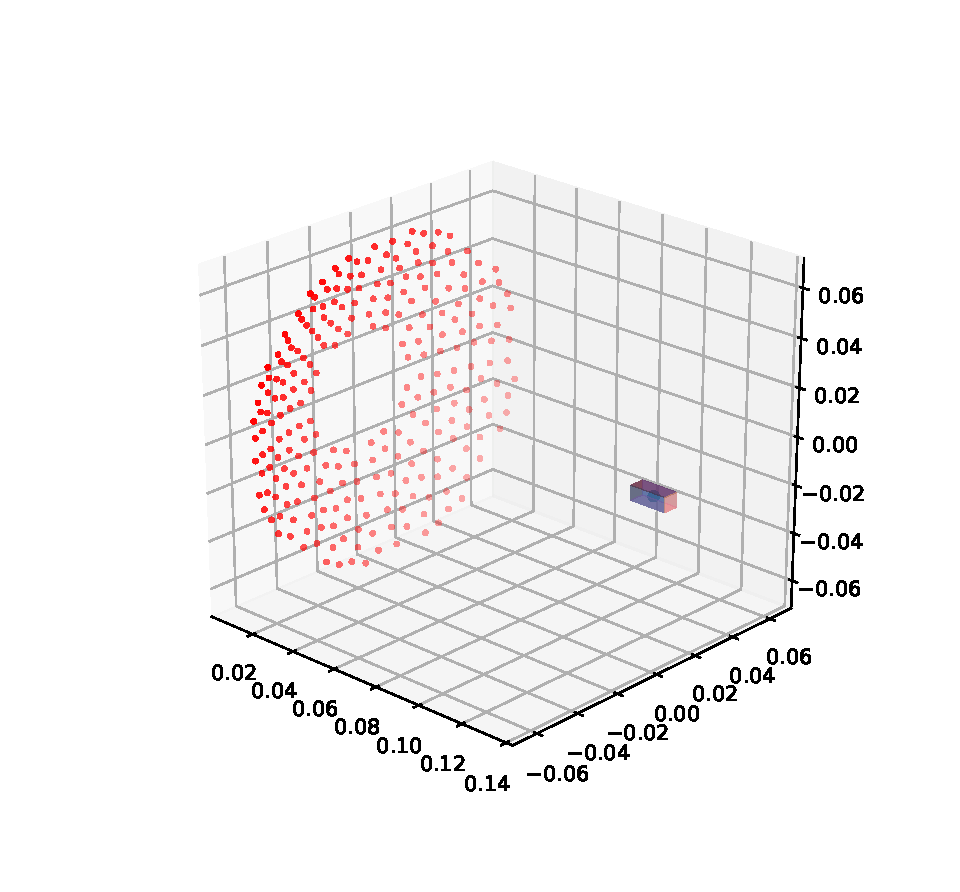
\includegraphics[width=0.6\textwidth]{sampling_box}
    \caption{Sampling box around the focus point with positions of the transducer elements.}
    \label{fig:sampling_box}
\end{figure}

As explained in Section \ref{sec:trident_theory}, a trident ray in this model consists of three closely aligned rays. One ray carrys the power and is referred to as "power ray". The other two rays only help to determine the divergence of the beam and are referred to as "auxiliary ray". The angle between any two rays of the three is referred to as "trident angle".

%%%%%%%%%%%%%%%%%%%%%%%%%%%%%%%%%%%%%
\section{Implementation of the Model} \label{sec:implement}
The mathematical model is written in the Python programming language, using scipy suite\cite{scipy}. The visualization of the model is made possible with matplotlib \cite{matplotlib}. The model is produced as a python package \texttt{pyHIFU} and is available online. The four components mentioned in section \ref{sec:components} will be introduced in detail. A Python class is implemented for these four component. This make the program more intuitive and easy to maintain. Other than these four component, the geometry and acoustics are also implemented in an object-oriented manner. The class \texttt{HIFU} encapsulates several methods for manipulating the four components above. As is shown in Figure \ref{fig:uml_overview}, \texttt{transducer} casts \texttt{ray} at \texttt{media}. The rays are grouped into bundle according to their wave type and media history. Then, \texttt{box} samples the intensity generated by every bundle to get the resultant pressure. The same routine is run for all the transducers. The final result is the summation of the result from all transducers. Initialization of the model requires a lot of parameters, a json document is used as configuration file to simplify passing parameters.

\begin{figure}[h]
    \centering
    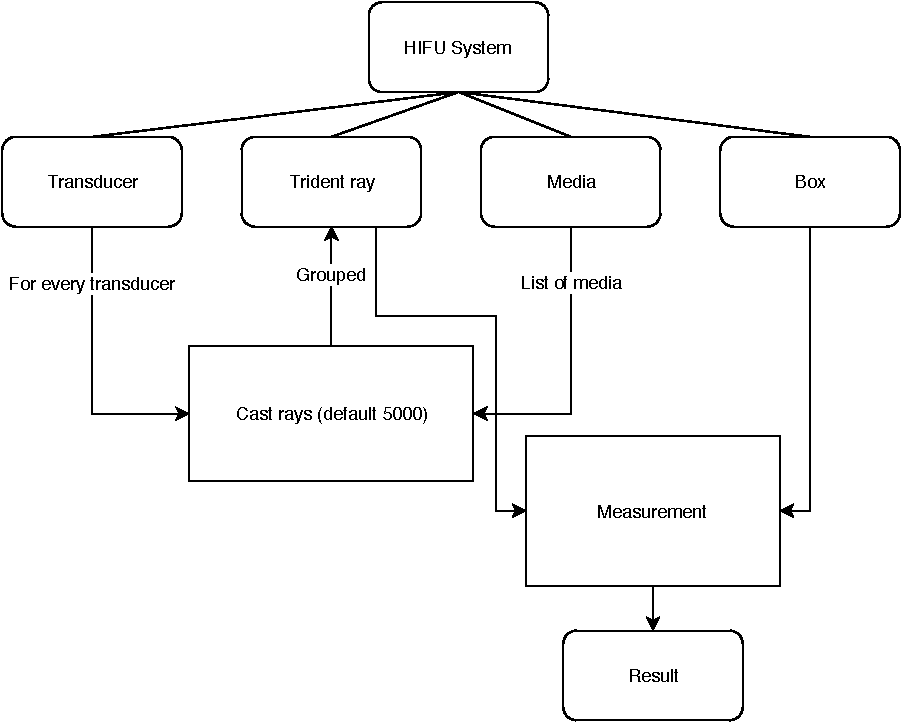
\includegraphics[width=0.8\textwidth]{uml_overview}
    \caption{An overview of all the components in the HIFU system.}
    \label{fig:uml_overview}
\end{figure}

%%%%%%%%%%%%%%%%%%
\subsection{Media} \label{sec:Media}
A medium is implemented in class \texttt{Medium}. The medium in this study mainly consists of two parts, geometry and material. The geometry of the medium is an instance of the shape in module geometry (Appendix \ref{ap:geometry}) and defines the shape of the medium in 3D space. The material of the medium defines the physical properties of the medium, including all the properties in Table \ref{tb:media_property}. For example, a medium can have the cuboid as its geometry and the bone as its material. Some properties such as the speed of sound and the attenuation in solid media have different values for longitudinal waves and shear waves. These properties would be stored as a list with the first element as the property of longitudinal waves and the second element the property of shear waves. A shape contains several faces. For example, the shape of a cylinder is composed of two circles and a barrel shape. These faces are organized as a list and each of them has its own ID. When a instance of a geometry is initialized, a matrix is created as its property to store the topological relationship of the shape. A typical such matrix of a cylinder would be

\[
\begin{bmatrix}
    None & 0 & None \\
    0 & None & 1 \\
    None & 0 & None
\end{bmatrix}
\]

For example, the first element of the second row is $0$ because the barrel shape is adjacent to the upper circle on its first (index 0) edge. The two circles are not adjacent, thus the corresponding elements are $None$.

A Model can contain several media. They can be identified with their \texttt{ID}. The media are stored in a graph structure named \texttt{MediaComplex}. For example, in the simplest case, the only medium in the system is Castor oil \textit{medium 0}. If muscle is taken into consideration, \textit{medium 0} would be Castor oil and \textit{medium 1} muscle. The \texttt{MediaComplex} is implemented such that the first element is always Castor oil or any other initial medium. When a ray travels in a medium, it is important to be able to determine the next medium so as to calculate the percentage of the power that is transmitted and reflected to the various ray types. The graph structure in this model is implemented as a list with an adjacency matrix \texttt{adj\_mtx}. The adjacency matrix is a square matrix $M$. $M_{i,j}$ is the index of the face (Appendix \ref{ap:geometry}) of \textit{medium i} that is adjacent to \textit{medium j}. In this study, the media all have a cubiod shape. It can be extended to more complex shapes such as cylinders or spheres with a little effort.

\begin{figure}[h]
    \centering
    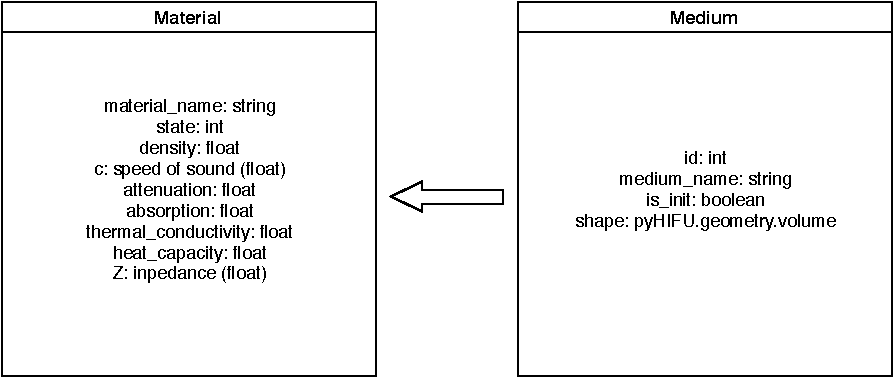
\includegraphics[width=0.8\textwidth]{uml_cls_media}
    \caption{Inheritance relation between class Medium and class Material.}
    \label{fig:uml_cls_media}
\end{figure}

%%%%%%%%%%%%%%%%%%%%
\subsection{Trident} \label{ssec:trident}
As mentioned earlier, the ray that carries power is implemented as class \texttt{PowRay} (power ray) and the ray that only helps to determine the divergence is implemented as class \texttt{AuxRay} (auxiliary ray). They both inherit from a general purpose ray class \texttt{Ray}. Acoustic rays in this model are represented as geometrical rays \texttt{pyHIFU.geometry.Ray}. Class \texttt{Ray} is a subclass of the geometrical ray class \texttt{GeoRay} (Appendix \ref{ap:geometry}), adding some properties and methods for acoustics simulation.

A trident ray (class \texttt{Trident}) consists of three rays, one \texttt{PowRay} and two \texttt{AuxRay}s. Every trident has a unique id. Interaction with media doesn't change the id. Member property \texttt{el\_id} stores the id of the transducer where it is cast from. The trident class also contains the reference to the media that it resides in. The member property \texttt{history} records all the media that trident ray has passed through. \texttt{wavetype} is an integer variable that indicates whether the ray is longitudinal (0) or shear (1) wave. A ray can encounter several intersections with media interfaces and produce up to four child rays in case of solid-solid intersection. Each intersection splits the parent rays into reflected rays and transmitted rays, the power is divided over the rays according to the solutions to the acoustic Fresnel equations for the given situation. Once the power of the ray is lower than a predefined threshold \texttt{powerlimit}, the ray is discarded and the propagation stops.
The trident rays are grouped into bundles according to their \texttt{bundle\_identifier}. The \texttt{bundle\_identifier} is a string that is composed of the id of the transducer the ray originates from, its history and its wavetype. For example, \texttt{tr\_128\_mh\_0\_1\_1\_1\_LONGIT} can be intepreted as a longitudinal trident ray cast from transducer element \textit{no.128} propagating from \textit{media 0} into \textit{media 1} then reflected inside  \textit{media 1} twice until its power is lower than \texttt{powerlimit}.

\begin{figure}[h]
    \centering
    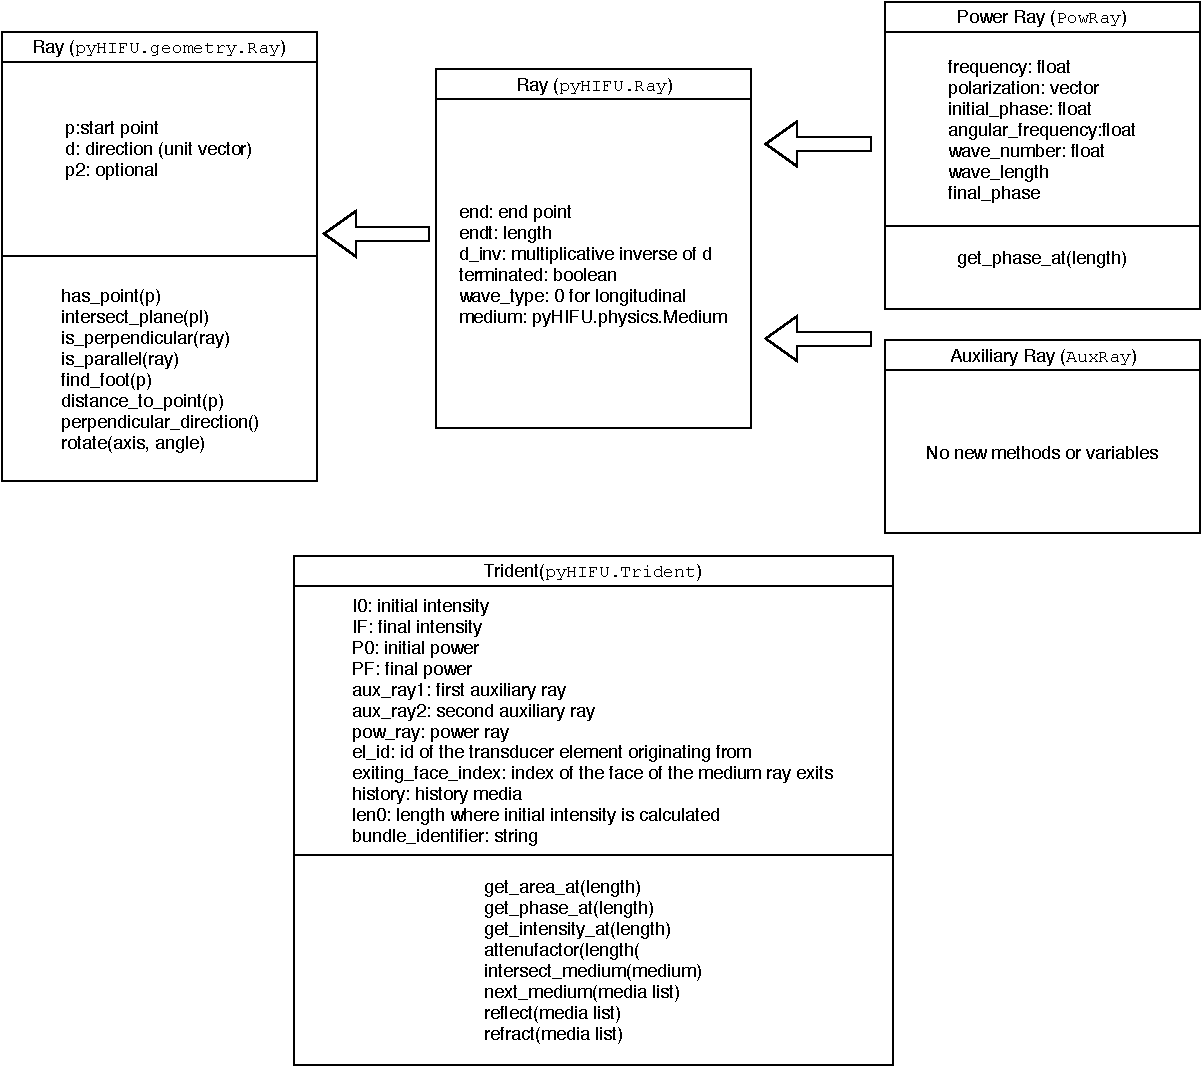
\includegraphics[width=0.9\textwidth]{uml_cls_trident}
    \caption{Relation among class \texttt{pyHIFU.geometry.Ray}, \texttt{Ray}, \texttt{PowRay}, \texttt{AuxRay}  and  \texttt{Trident}.}
    \label{fig:uml_cls_trident}
\end{figure}

Ideally, the pressure profile of the ultrasound field in the far-field and near-field can be predicted using the wave equations \cite{vanwijk2013}. However, the difficulty arises due to rising computational cost with increasing geometrical complexity when using the classic finite element or boundary element approach. In this simulation, only if a trident is cast from a transducer element, not generated by reflection or refraction, is its initial intensity determined by the far-field approximation of the ultrasound profile (Section \ref{sec:measurement}). Otherwise, the initial intensity is determined using Fresnel's equations. There's a minimal distance for a far-field approximation to hold \cite{auld1973acoustic}. This distance is referred as $D_z$ in this study. It is a intrinsic property of the transducer elements.

\begin{equation} \label{eq:distancz}
    D_z=\frac{2.3 \cdot r_t}{\lambda}
\end{equation}

$r_t$ is the radius of the transducer element and $\lambda$ is the wave length of the ultrasound. The initial phase of all rays from the transducer element is 0. When initializing a trident ray, the initial pressure is calculated from the far-field approximation at $D_z$. The initial intensity is calculated from equation \ref{eq:intensity_from_pressure}.

\begin{subequations}
    Conversion between intensity and power:
    \begin{align} 
        I_0 = \frac{pressure^2}{2 \cdot Z} \label{eq:intensity_from_pressure}\\
        P_0 = I_0 \cdot Area(D_z) \label{eq:power_from_intensity}\\
        P_{r} = P_0 \cdot e^{-2 \alpha r} \label{eq:power_decay}\\
        I_{r} = \frac{P_r}{Area(r)} \label{eq:intensity_from_power}
    \end{align}
\end{subequations}

After initialization, the far-field approximation is no longer used. The area formed by the three rays is affected by the solid angle (trident angle) and so is the initial power \ref{eq:power_from_intensity}. The area in equation \ref{eq:intensity_from_power} increases quadratically as the distance from the origin of the ray increases. Hence, the intensity decreases quadratically due to beam spreading and exponentially due to attenuation. 

\begin{figure}[h]
    \centering
    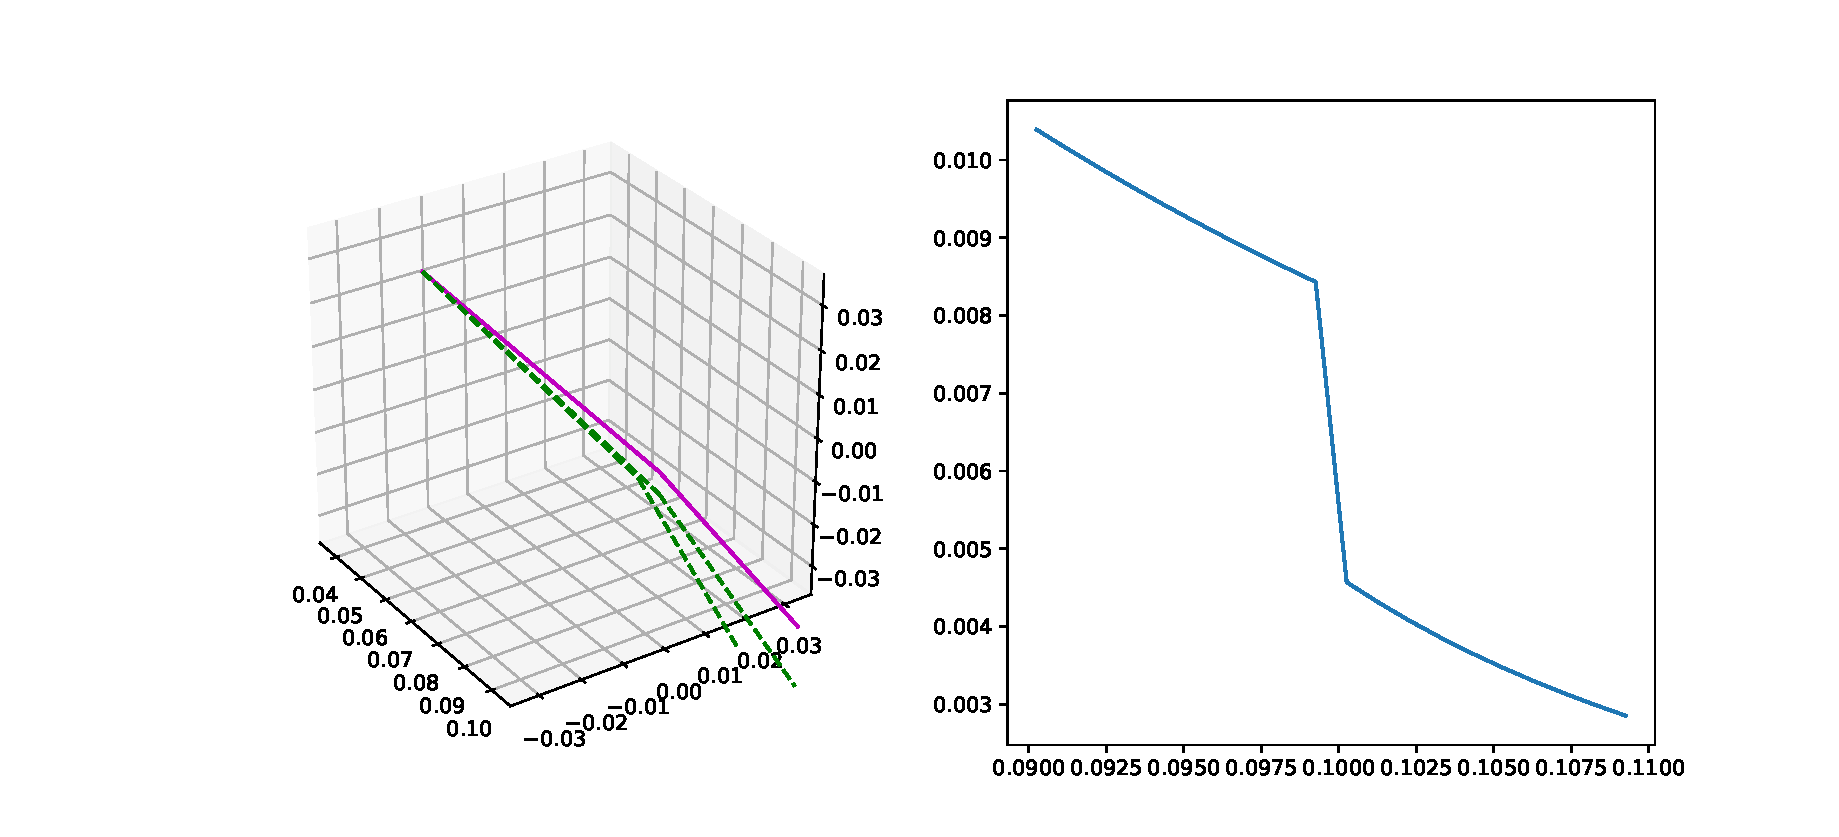
\includegraphics[width=0.8\textwidth]{intensity_plot_at_refraction2}
    \caption{The intensity change along a trident ray  with one refraction. The green dash lines are auxiliary rays and the magenta ray is the power ray. The turning point on the ray is the position of the interface (left). As can be observed in the figure, the intensity first changes exponentially, then decreases suddenly after the intersection with media interface at $0.1$ m (right). After the intersection, the intensity again changes exponentially according to the attenuation equation.}
    \label{fig:intensity_plot_at_refraction2}
\end{figure}

$P_0$ in equation \ref{eq:power_from_intensity} is derived from real intensity $I_0$ from the far-field approximation and spreading area $Area$. Equation \ref{eq:intensity_quadratically} shows that the intensity of a trident decreases quadratically with length, with exponential attenuation. Although power is affected by trident solid angle, the intensity is not determined by the trident solid angle at all.

\begin{equation} \label{eq:intensity_quadratically}
    \begin{aligned}
        I_r &= \frac{P_0}{Area(r)} \cdot e^{-2 \alpha r} \\
        &= \frac{I_0 \cdot Area(D_z)}{Area(r)} \cdot e^{-2 \alpha r} \\
        &= I_0 \cdot \left(\frac{D_z}{r}\right)^2 \cdot e^{-2 \alpha r}
    \end{aligned}
\end{equation}

When the ray travels inside a bounded media, it eventually encounters the boundaries of the media. To calculate the direction of new rays, some properties of the new medium are required. As explained in Section \ref{sec:Media}, the media are stored as a graph. The method \texttt{next\_medium} of class \texttt{Trident} locates the next medium by looking up the adjacency matrix. A trident ray contains three rays. Each of these rays intersect with the boundaries and produces their child rays. These child rays are grouped into a new trident after intesection, i.e., reflected longitudinal power ray and reflected longitudinal auxiliary rays are grouped into a new reflected longitudinal trident (Figure \ref{fig:interaction_of_trident}). If auxiliary intersects outside the interface, the interface is expanded as an infinite plane to guarantee that the auxiliary rays and the power ray in the same trident should always intersect the same interface.

\begin{figure}[h]
    \centering
    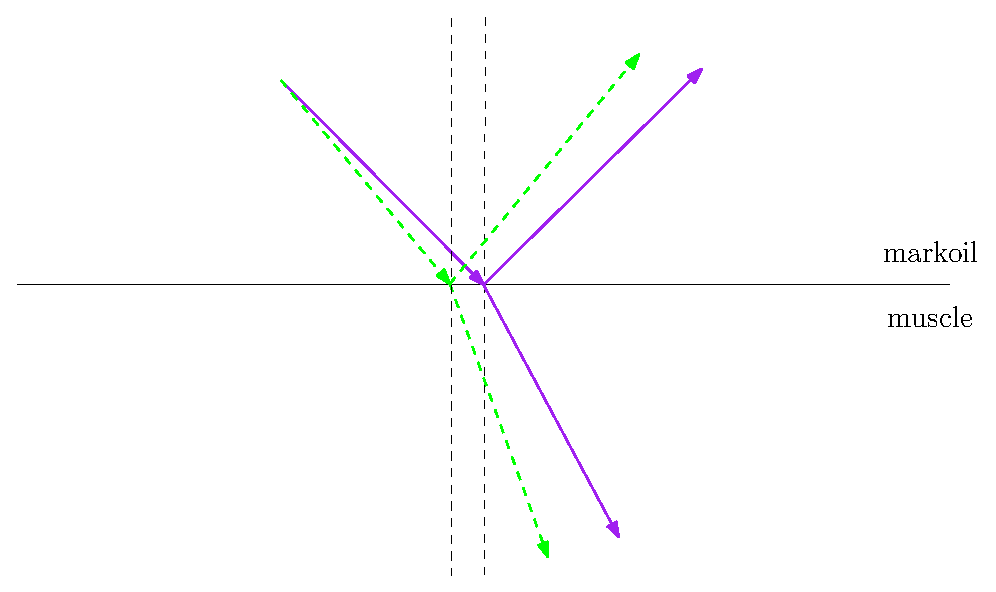
\includegraphics[width=0.6\textwidth]{interaction_of_trident}
    \caption{The purple ray is a power ray and the green dashed line is an auxiliary ray. For simplicity, only one auxiliary ray is displayed. Every interaction of a trident with an interface gives rise to three new rays which will make up a new trident.}
    \label{fig:interaction_of_trident}
\end{figure}


%%%%%%%%%%%%%%%%%%%%%%%
\subsection{Transducer}
A transducer element is a device that can convert other forms of energy into acoustic energy in the form of ultrasound. The transducer in this study consists of 256 transducer elements. In the model, the transducer is implemented as class the \texttt{Transducer} and the transducer element is implemented as the class \texttt{TElement}. \texttt{Transducer} maintains a list of instances of the class \texttt{TElement}, in this case, the length of the list is 256.
Every transducer needs to cast rays and group them according to its bundle identifier string. This is implemented as a Python dictionary of which the keys are the bundle identifier string. As mentioned earlier, rays are discarded if their power is lower than power limit. In this model, the power limit is defined as $0.1\%$ of the initial power. 

\begin{figure}[h]
    \centering
    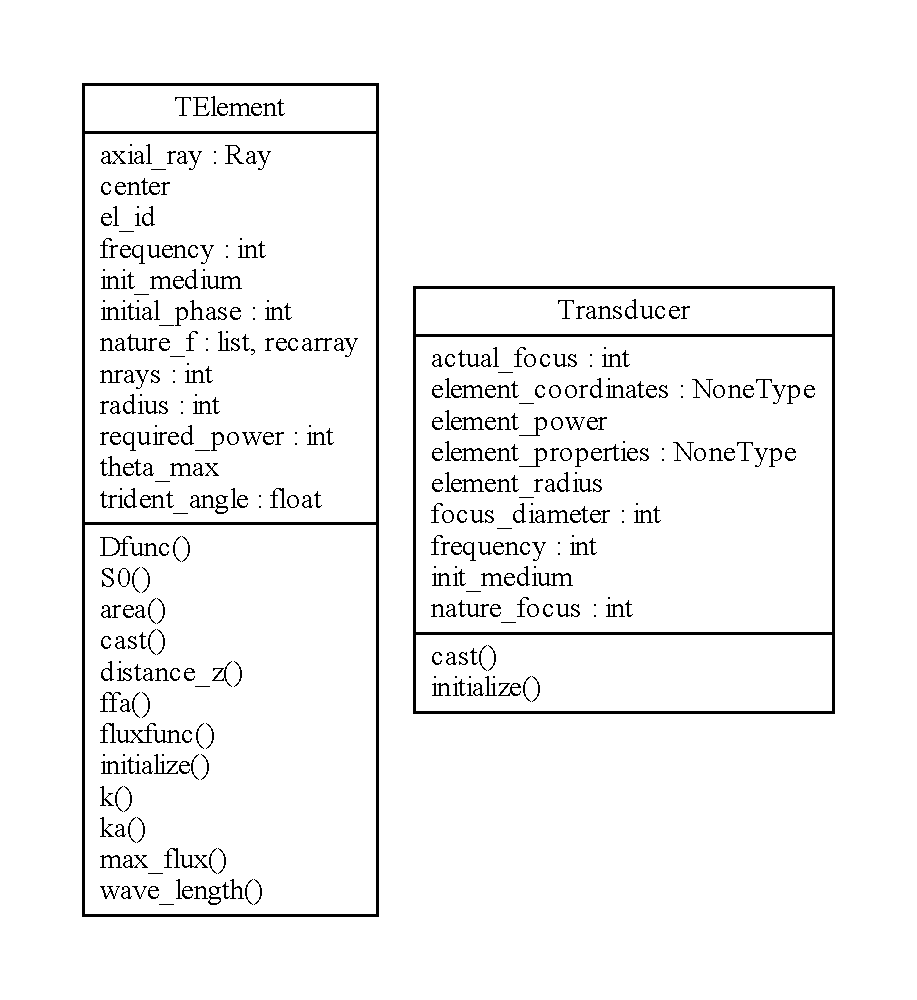
\includegraphics[width=0.6\textwidth]{uml_cls_transducer}
    \caption{Class \texttt{pyHIFU.transducer.Transducer}, \texttt{pyHIFU.transducer.TElement}.}
    \label{fig:uml_cls_transducer}
\end{figure}

\IncMargin{1em}
\begin{algorithm}[H]
    \DontPrintSemicolon
    \SetKwInOut{Input}{input}\SetKwInOut{Output}{output}
    \Input{$nray$: number of the rays from one transducer, $trident\_angle$: angle between \texttt{AuxRay} and \texttt{PowRay}, $\theta_{max}$: the maximum angle from the axis of a transducer element to cast rays.}
    \Output{bundles: dictonary with the bundle identifier string as the key}
    $bundles \leftarrow$ empty dictionary\;
    $total\_ray\_number \leftarrow 0$\;
    \For{$i\leftarrow 1$ \KwTo $nray$}{
        $\theta_i \leftarrow$ random angle between $0$ and $\theta_{max}$\;
        $\beta_i \leftarrow$ random angle between $0$ and $2\pi$\;
        $p_i \leftarrow$ point on polar coordinate defined by $\theta_i$ and $\beta_i$\;
        $tr_i \leftarrow$ trident at the direction of $p_i$\;
        $queue \leftarrow$ empty queue\;
        append $tr_i$ to $queue$\;
        \While{$queue$ is not empty}{
            $tr \leftarrow$ $queue$ pop from left\;
            \uIf{the power of $tr$ is less than powerlimit}{discard $tr$\;}
            \Else{
                put $tr$ into $bundles$\;
                append reflected rays of $tr$ to $queue$\;
                append refracted rays of $tr$ to $queue$\;
            }
        }
    }
    \Return $bundles$
    \caption{Casting rays from one transducer element}\label{algo_disjdecomp}
\end{algorithm}
\DecMargin{1em}

The operation on every transducer element is independent from each other. Multiprocessing is employed to accelerate the simulation process, with each transducer being handled by one process. The result from every transducer element is summed to yield the final result (equation \ref{eq:sum_pressure}).

%%%%%%%%%%%%%%%%%%%%%%%%%
\subsection{Sampling box}
Only the area around focus point of the HIFU system is measured in this model. Box defines an "axis-aligned bounding box" in the geometry where the pressure will be measured (Figure \ref{fig:sampling_box}). It is divided into smaller cubes implemented in the class \texttt{Lattice} (Figure \ref{fig:gridbox}).

\begin{figure}[h]
    \centering
    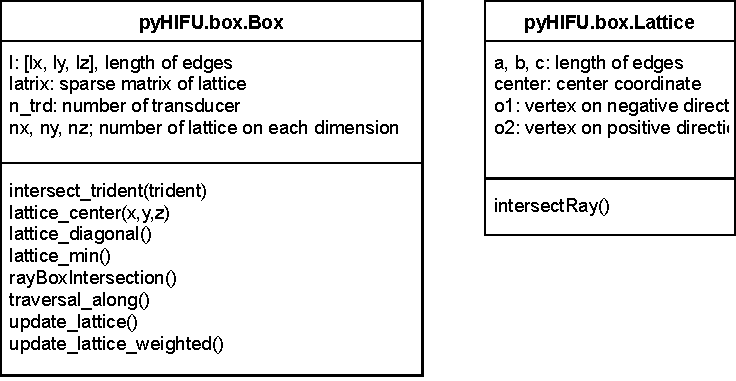
\includegraphics[width=0.6\textwidth]{uml_cls_box}
    \caption{Components of the class Box and the class Lattice.}
    \label{fig:uml_cls_box}
\end{figure}

\texttt{Box} takes a function handle as its argument. When the sampling box traverses along a trident ray,  it performs updates to all the intersected cubes using this function handle. In this study, the sampling method uses the ratio of the length of intersection segment and the cube diagonal as the weight for intensity contribution. In section \ref{sec:ray_tracing} and \ref{sec:measurement}, it will be further illustrated. 

\begin{figure}[h]
    \centering
    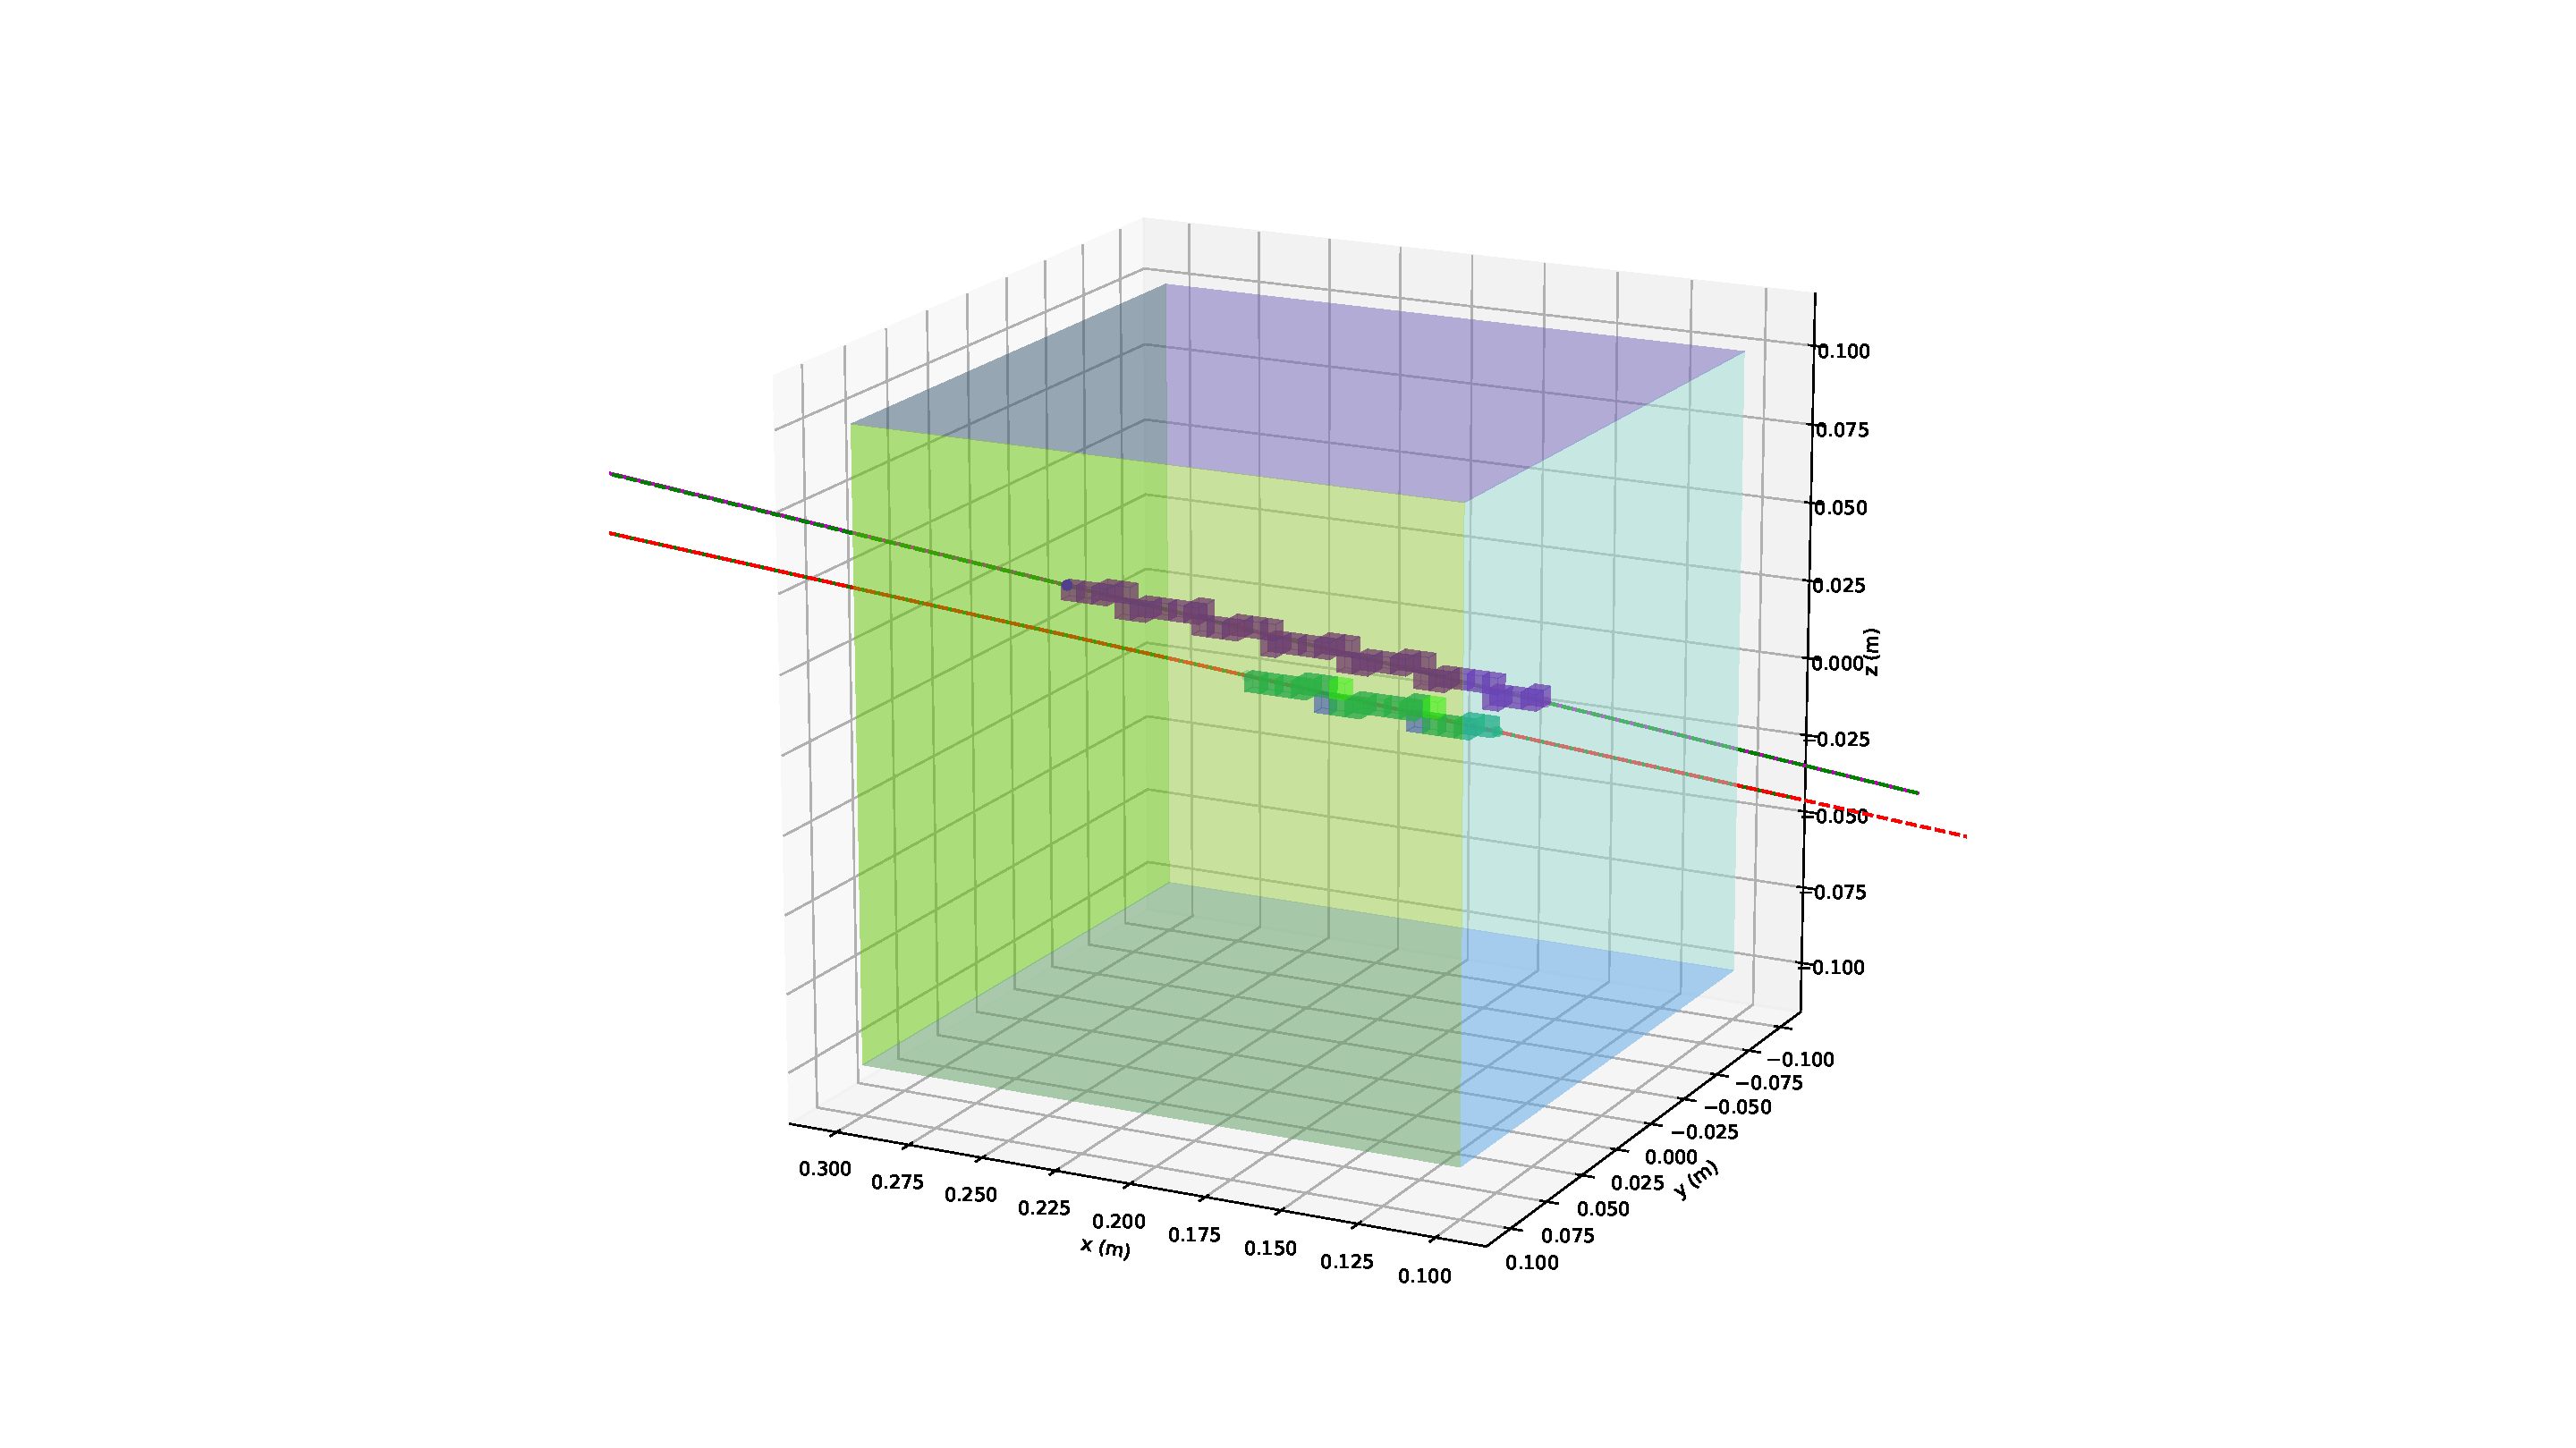
\includegraphics[width=\textwidth]{box_intersection}
    \caption{Box intersecting with two trident rays in two directions (forward and backward). The cubes that intersects the ray in different directions are displayed in different colors.}
    \label{fig:box_intersection}
\end{figure}

%%%%%%%%%%%%%%%%%%%%%%%%%%%%%%%%%%%%%
\section{Reflection and Transmission} \label{sec:rnr}

When a ray travels in the geometry, it encounters media interfaces and is reflected and refracted. Considering the trident ray (Section \ref{ssec:trident}) in this model, we simply perform reflection and refraction on both the power ray and the auxiliary rays. Shear waves can only travel in solid media while longitudinal waves can travel in both solid and fluid media, hence resulting in four types of interactions, fluid-fluid, solid-solid, fluid-solid and solid-fluid interactions (Figure \ref{fig:reflect_refract}). 
There are two laws used in the simulation of reflection and transmission: Snell's law that calculcates the direction of new rays and Fresnel's equations that calculates the energy distribution among the rays.

\begin{figure}[h]
    \centering
    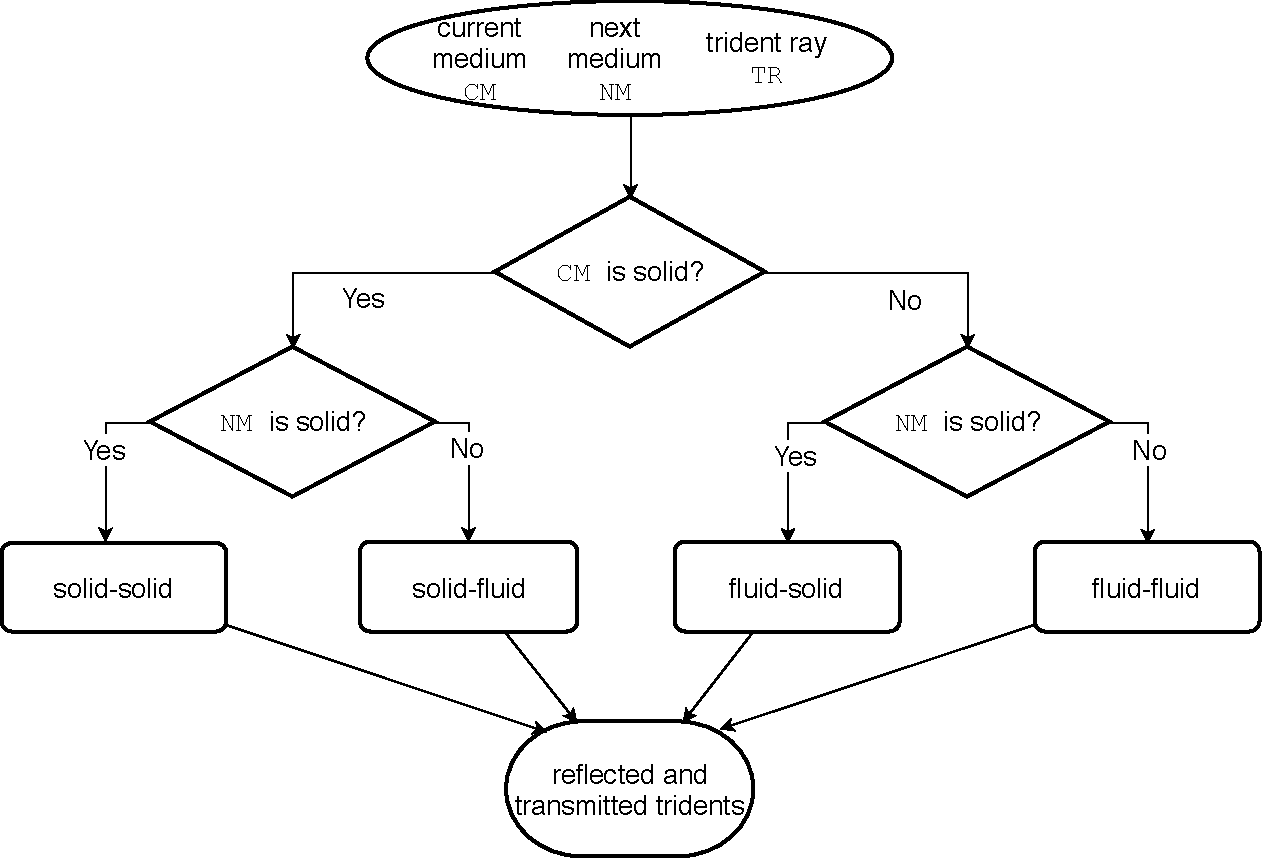
\includegraphics[width=0.9\textwidth]{reflect_refract}
    \caption{Flowchart of reflection and transmission}
    \label{fig:reflect_refract}
\end{figure}

Fluid-fluid interaction is the most simple one among the four types. In a fluid medium, only longitudinal waves can propagate. The reflected ray and transmitted ray are longitudinal only. Solid-solid interaction is a more complicated situation since it also needs to consider the polarization directions. In this model, only the fluid-fluid interface is implemented and tested because of its simplicity. Future work will include implementing the functionality of shear wave reflection and refractions.

For both reflection and refraction, the direction of the new rays are determined by Snell's law (Equation \ref{eq:snells}). $\theta_x$ refers to the angle between $\vec{n}$ and reflected rays or the angle between $-\vec{n}$ and transmitted rays as shown in Figure \ref{fig:inter_ss}. If the reflected ray and the incident ray have the same wave type, i.e., they are both longitudinal or shear waves, the reflection angle $\theta_{r}$ is equal to the incident angle $\theta_i$.The speed of longitudinal wave and shear wave are different in the same medium. If they have different wave types, according to equation \ref{eq:snells}, the two angle should also be different.

\begin{equation} \label{eq:snells}
    \frac{sin(\theta_i)}{sin(\theta_{x})} = \frac{c_1}{c_2}=\eta
\end{equation}

\begin{figure}[h]
    \centering
    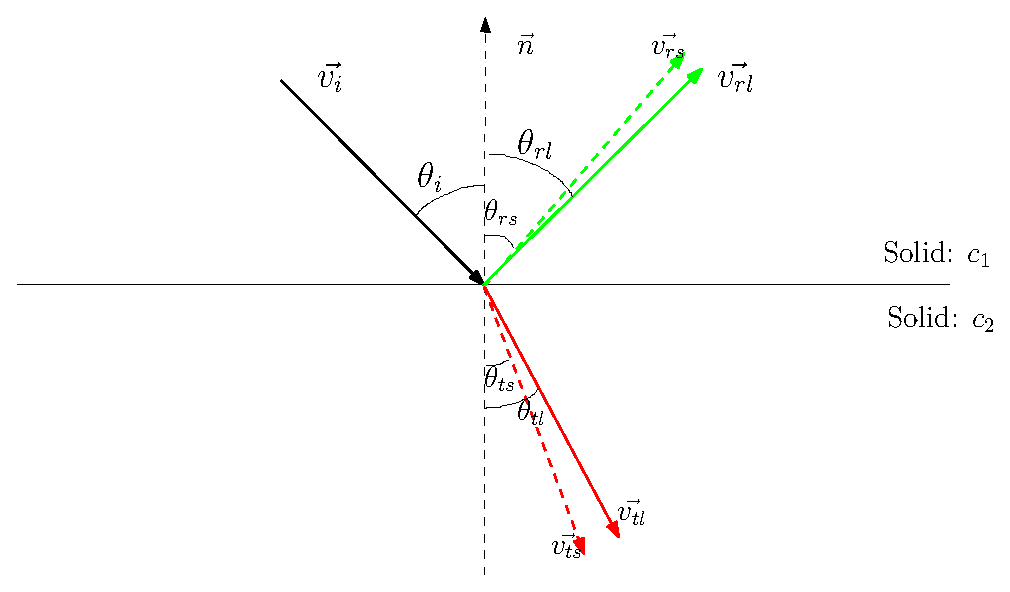
\includegraphics[width=0.6\textwidth]{inter_ss}
    \caption{Reflection and transmission at a solid-solid interface}
    \label{fig:inter_ss}
\end{figure}

%%%%%%%%%%%%%%%%%%%%%%%%%%%%%%%%
\section{Ray Tracing Simulation} \label{sec:ray_tracing}

The algorithm to trace the ray in the sampling box developed in this study is a variant of Bresenham line drawing algorithm \cite{bresenham} but for 3D geometry. It is implemented as a class method of \texttt{pyHIFU.box.Box}. The algorithm can be divided into two phases: initialization and incremental traversal. To make it more intuitive, the algorithm is illustrated in 2-dimension first. Consider Figure \ref{fig:traversal_along}, the algorithm should visit the voxels in the same order as their labels \cite{wooraytracing}.

\begin{figure}[h]
    \centering
    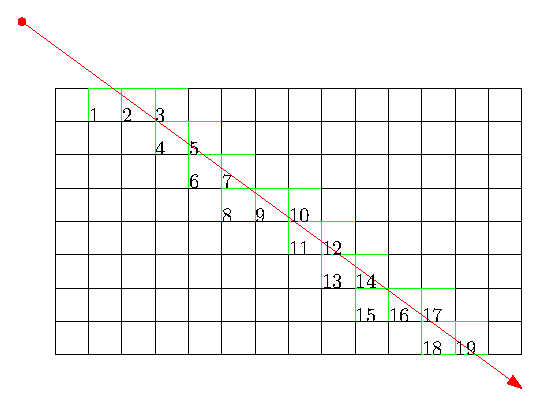
\includegraphics[width=0.6\textwidth]{traversal_along}
    \caption{A ray intersects a 2D raster, green square indicating the interaction.}
    \label{fig:traversal_along}
\end{figure}

The initialization phase finds the coordinates and voxels where the intersection with the box starts and ends, in Figure \ref{fig:traversal_along} it is voxel 1 and voxel 19 respectively \cite{smits}. If the ray doesn't intersect the box, the ray is not processed. If the ray intersects the box, there are two situation to consider: whether the ray starts or ends inside the box or not. The routine (Appendix \ref{ap:rayboxintersection}) for calculating the intersection of the ray with the box returns the distances from the two intersection points to the origin of the ray, in this report the distance from the start of intersection is referred to as $st$, the distance from the end of the intersection as $et$. For example, $st$ and $et$ are the distance from the origin of the ray to the first and last horizontal lines in Figure \ref{fig:traversal_along}, respectively. From the formula of the ray and $st$ and $et$, the coordinate of the starting cube \texttt{[X, Y, Z]} and the coordinate of the ending cube \texttt{[X2, Y2, Z2]} can be determined (Appendix \ref{ap:floatnumber}). Variables \texttt{StepX, StepY, StepZ} are initialized to $1$ if their direction is incremental and $-1$ otherwise. Next, we compuate variables \texttt{tDeltaX, tDeltaY, tDeltaZ}. \texttt{tDeltaX} is the distance to move along the ray between two adjacent $y-z$ planes, similarly for \texttt{tDeltaY} and \texttt{tDeltaZ}. Finally we compute the distance to move along the ray from the origin of the ray to the next $y-z$ plane as \texttt{tMaxX}, again similarly for \texttt{tMaxY} and \texttt{tMaxZ}.

The incremental phase is similar to other digital differential analyzer algorithms. It keeps track of the variables \texttt{tMaxX, tMaxY, tMaxZ} and updates them with every increment of \texttt{[X, Y, Z]}, the coordinate of the axis-aligned bounding boxes system within the sampling box. \texttt{tMaxX, tMaxY, tMaxZ} indicates the plane where the closest intersection point is located. For example, if \texttt{tMaxX} is the smallest among the three, the ray should intersect the next cube on the $x$ direction. First, increment to \texttt{[X, Y, Z]} is performed according to \texttt{tMaxX, tMaxY, tMaxZ}. After the increment on coordinate, the corresponding distance (\texttt{tMaxX, tMaxY, tMaxZ}) should be updated to the distance of the next plane in its corresponding direction. For the $x$ direction, \texttt{tMaxX} should be incremented by \texttt{tDeltaX}. Algorithm \ref{algo:increment} demonstrates the incremental phase in 3D geometry. This algorithm is a strictly adjacency ray tracing algorithm. The boxes have to have common face to be considered adjacency. The algorithm always favours the box closer to the ray direction if the ray intersects right at the box edge.

Due to the precision of float number, the coordinates of the intersection points calculated from the algorithm does not always mathematically perfectly sit on the cubes. A routine to handle this problem is addressed in Appendix \ref{ap:floatnumber}.

\IncMargin{1em}
\begin{algorithm}[H] \label{algo:increment}
    \DontPrintSemicolon
    \While{not reached the end \texttt{[X2, Y2, Z2]}}{
        process \texttt{[X, Y, Z]} using the \emph{function handle}\;
        \uIf{tMaxX $<$ tMaxY}{
            \uIf{tMaxX $<$ tMaxZ}{
                tMaxX = tMaxX + tDeltaX\;
                X = X + stepX\;
            }
            \Else{
                tMaxZ = tMaxZ + tDeltaZ\;
                Z = Z + stepZ\;
            }
        }
        \Else{
            \uIf{tMaxY $<$ tMaxZ}{
                tMaxY = tMaxY + tDeltaY\;
                Y = Y + stepY\;
            }
            \Else{
                tMaxZ = tMaxZ + tDeltaZ\;
                Z = Z + stepZ\;
            }
        }
    }
    \caption{Incremental phase of the ray tracing algorithm}
\end{algorithm}
\DecMargin{1em}


%%%%%%%%%%%%%%%%%%%%%
\section{Measurement} \label{sec:measurement}
Measurement is conducted after the ray casting process is finished. \texttt{cast} method from transducer element class \texttt{TElement} returns a dictionary where the rays are sorted according to their \texttt{bundle\_identifier}. There are two variables that are required to calculate the final result, average intensity of a bundle, average phase of a bundle. First, the rays are sampled on the sampling box in bundles. For every ray $r_i$ in bundle $B_i$, the sampling routine goes as follows:

\IncMargin{1em}
\begin{algorithm}[H] \label{algo:sampling}
    \DontPrintSemicolon
    pc = zeros(dimension of box)\;
    \tcc{pressure (complex number)}
    \ForEach{bundle $B$}{
        $I$ = zeros(dimension of box)\;
        $ph$ = zeros(dimension of box)\;
        $counter$ = zeros(dimension of box)\;
        \ForEach{ray $r \in B$}{
            update $I$\;
            update $ph$\;
            update $counter$\;
        }
        \ForEach{coordinate $[x,y,z]$ in $I$}{
            pc+=$\sqrt{\frac{2\cdot Z\cdot I(x,y,z)}{N_B}} \cdot e^{\frac{i\cdot\phi}{N}}$\;
        }
    }
    \caption{Sampling routine of one bundle $B$}
\end{algorithm}
\DecMargin{1em}

The pressure caused by one bundle $B$ to a cube \texttt{(x, y, z)} is

\begin{equation} \label{eq:sum_pressure}
    pressure = \sum_{tr\in B} \sqrt{\frac{2\cdot Z\cdot I(x,y,z)}{N_B}} \cdot e^{\frac{i\cdot\phi}{N}}
\end{equation}

$Z$ is the attenuation factor, $N_B$ is the number of trident rays in bundle $B$.

There are two methods to update the intensity $I$ in the first loop in Algorithm \ref{algo:increment}. Consider in the Figure \ref{fig:measure}, the first method is to find the perpendicular foot $F$ of the center $C$ of the box on ray $\vec{AB}$. The intensity at point $F$ is used as the contribution of this ray to the box. The secound method is a weighted contribution of the intensity. First, the intensity $I_F$ at point $F$ is measured in the same way as in the first method. Then, the length of the intersection of the ray with the box $|AB|$ is calculated. The contribution of the ray $\vec{AB}$ to the box would be $I_F \cdot \frac{|AB|}{D}$ where $D$ is the length of the diagonal of the box.

\begin{figure}[h]
    \centering
    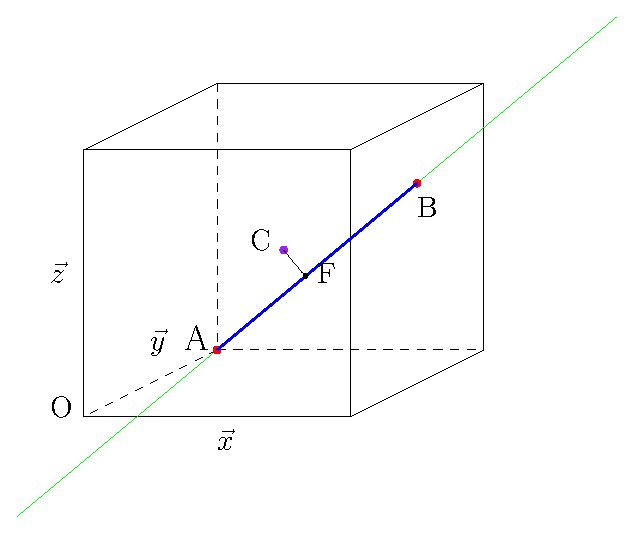
\includegraphics[width=0.5\textwidth]{measure}
    \caption{Ray intersection with a cube. $A$: entry point, $B$: exit point, $C$: center of the cube, $O$: lowest point of the cube, $F$: perpendicular foot on ray through $C$, $CF \perp AB$.}
    \label{fig:measure}
\end{figure}

Errors are introduced to the result when using ratio of the length of the intersection segment to the length of cube diagonal as the weight. The resulted intensity is not in SI unit \cite{unitscale}. However, we still can compare the result with the other simulation methods (Section \ref{sec:results}). This study only focus on the simulation of longitudinal wave in fluid media with one interface.


